% Author : Alexandre Quenon
% Last update : Décembre 2020 by Ibraimovski Roméo

% % % % % % %
%  Packages %
% % % % % % %

%---Base packages
\documentclass[a4paper,12pt]{report}	% document type (article, report, book)
\usepackage[utf8]{inputenc}			% encoding
\usepackage[T1]{fontenc}			% accent
\usepackage{lmodern}				% latin font
\usepackage{appendix}				% to be able to use appendices
\usepackage{float}

%---Language(s)
\usepackage[english,frenchb]{babel}	% last language = typography by default
\addto\captionsfrench{				% to change the french names of...
	\renewcommand{\appendixpagename}{Annexes}	% (default Appendices)
	\renewcommand{\appendixtocname}{Annexes}	% (default Appendices)
	\renewcommand{\tablename}{\textsc{Tableau}}	% (default \textsc{Table})
}

%---Page layout
%------> margins
	% 1st option -> geometry package
		%\usepackage[a4paper]{geometry}		% default parameters for A4
		%\usepackage[top=2in, bottom=1.5in, left=1in, right=1in]{geometry}
	% 2nd option -> a4wide package
		\usepackage{a4wide}		% A4 with smaller margins (the one I've chosen)
	% 3rd option -> fullpage package
		%\usepackage{fullpage}
%------> chapter style
	% 1st option -> fncychap package
		%\usepackage[style]{fncychap}		% style = Lenny, Bjornstrup, Sonny, Conny
	% 2nd option -> customized styles
		%
%------> cover page (UMONS template)
	\usepackage[fs]{umons-coverpage}		% NEED "umons-coverpage.sty" file
	\umonsAuthor{Made by Roméo \textsc{Ibraimovski} \& Maxime \textsc{Nabli}}
	\umonsTitle{Rapport de projet}
	\umonsSubtitle{Rapport Final}
	\umonsDocumentType{S-INFO-820	Projet de structures de données II}
	\umonsSupervisor{Supervised by Gauvain \textsc{Devillez}}
	\umonsDate{3e Bachelier en Sciences Informatiques\\ Année 2021-2022}

%---Numbering
\setcounter{secnumdepth}{2}			% numerotation depth (1=sec and all above)
\setcounter{tocdepth}{2}			% table of contents depth (1=sec and above)

%---Mathematics
\usepackage{amsmath}				% base package for mathematics
\usepackage{amsfonts}				% base package for mathematics
\usepackage{amssymb}				% base package for mathematics
%\usepackage{amsthm}				% theorem and proof environments
%\usepackage{cases}					% numcases environment
%\usepackage{mathrsfs}				% \mathscf command ('L' of Laplace-Transform,...)

%---Floating objects (images, tables,...)
\usepackage{float}					% better management of floating objects
\usepackage{array}					% better management of tables
\usepackage{graphicx}				% to include external images
\graphicspath{{Images/}}			% to put images in an 'Images' folder 
%\usepackage{caption}				% /!\ has priority on "memoir" class
%\usepackage{subcaption}			% subfigure and subtable environments
%\usepackage{subfig}				% \subfloat command
%\usepackage{wrapfig}				% wrapfigure environment
%\usepackage[update]{epstopdf}		% to use '.eps' files with PDFLaTeX

%---Code including
\usepackage{listings}				% general package (can be tuned)
%\usepackage[framed]{mcode}			% to include Matlab code
									% /!\ you need the "mcode.sty" file

%---Units from International System
\usepackage{siunitx}				% \SI{}{} command (units with good typography)
\DeclareSIUnit\baud{baud}			% definition of the "baud" unit
\DeclareSIUnit\bit{bit}				% definition of the "bit" unit

%---Drawing
%\usepackage{tikz}					% useful package for drawing
%\usepackage[european]{circuitikz} 	% to draw electrical circuits

%---Bibliography
\usepackage{url}					% to encore url
\usepackage[style=numeric-comp,backend=bibtex]{biblatex}
\usepackage{csquotes}				% inverted commas in references
%\bibliography{bibli}				% your .bib file

%---"hyperref" package				% /!\ it must be the last package
\usepackage[hidelinks]{hyperref}	% clickable links (table of contents,...)

%Pour écrire des algos: --------------------------------------------------------------------------
\usepackage{algorithmic, algorithm}

%Traduction en français
\floatname{algorithm}{Algorithme}
\renewcommand{\algorithmicrequire}{\textbf{Entrée :}}
\renewcommand{\algorithmicensure}{\textbf{Sortie :}}
\renewcommand{\algorithmicend}{\textbf{Fin}}
\renewcommand{\algorithmicif}{\textbf{Si}}
\renewcommand{\algorithmicthen}{\textbf{Alors}}
\renewcommand{\algorithmicelse}{\textbf{Sinon}}
\renewcommand{\algorithmicelsif}{\algorithmicelse\ \algorithmicif}
\renewcommand{\algorithmicendif}{\algorithmicend\ \algorithmicif}
\renewcommand{\algorithmicfor}{\textbf{Pour}}
\renewcommand{\algorithmicforall}{\textbf{pour tout}}
\renewcommand{\algorithmicdo}{\textbf{Faire}}
\renewcommand{\algorithmicendfor}{\algorithmicend\ \algorithmicfor}
\renewcommand{\algorithmicwhile}{\textbf{Tant que}}
\renewcommand{\algorithmicendwhile}{\algorithmicend\ \algorithmicwhile}
\renewcommand{\algorithmicloop}{\textbf{boucle}}
\renewcommand{\algorithmicendloop}{\algorithmicend\ \algorithmicloop}
\renewcommand{\algorithmicrepeat}{\textbf{répéter}}
\renewcommand{\algorithmicuntil}{\textbf{jusqu'à}}
\renewcommand{\algorithmicprint}{\textbf{imprimer}}
\renewcommand{\algorithmicreturn}{\textbf{Retourner}}
\renewcommand{\algorithmictrue}{\textbf{Vrai}}
\renewcommand{\algorithmicfalse}{\textbf{Faux}}
\renewcommand{\and}{\textbf{Et}}


%Enleve la numérotation des algorithmes
\makeatletter
\renewcommand{\fnum@algorithm}{\fname@algorithm}
\makeatother
%------------------------------------------------------------------------------------------------

% % % % % % %
% Document	%
% % % % % % %

\begin{document}

% Front matter
% ------------
%\frontmatter			% with class "book" only

	\umonsCoverPage		% produce the cover page with UMONS and your Faculty logo
	
	\pagenumbering{roman}	% if you don't use the class "book"
	
	\begin{abstract}	% environment adapted to write the abstract
Ce rapport d'implémentation est rendu dans le cadre de l'AA-S-INFO-820 ``Projet de structure de données II", supervisé par l'Assistant Gauvain Devillez en année académique 2021-2022. Ce rapport a pour but d'expliquer et de justifier nos différents choix de conception.
	\end{abstract}
	
	\clearpage			% to start the toc on a new page
	\tableofcontents
	%\clearpage			% to start the lof on a new page
	%\listoffigures
	%\clearpage			% to start the lot on a new page
	%\listoftables
	

% Main matter
% -----------
%\mainmatter			% with class "book" only

	\clearpage			% if you don't use the class "book"
	\pagenumbering{arabic}
	
	{\section*{Introduction}}
	\addcontentsline{toc}{chapter}{Introduction}	% to add in the toc
\noindent Dans le cadre des cours de "Structures de Données I" et "Structures de Données II" , nous avons vu les arbres binaires et
d'autres structures de données étant des variantes de ces Arbres. Pour ce projet du cours de "Structure de Données II",
nous avons du implémenter les "Binary Search Partition Tree", notés Arbres BSP pour le reste de ce rapport, structure de données
modelée après les arbres binaires. Ces Arbres BSP sont utilisés en géométrie pour représenter les objets contenus dans un plan.
Avec une droite, on coupe ce plan en 2 sous-plans, aussi appelés demi-espace ouvert positif ou négatif.
Le demi-espace ouvert positif est le sous-plan ou lorsque les coordonnées d'un point sont remplacée dans l'équation de la droite, on
a un résultat positif. Pareil pour le demi-espace ouvert négatif.
et, nous répétons cette action dans chacun des sous-plan crée jusqu'à ce qu'il ne reste qu'un fragment d'objet par sous-plan.
Les noeuds internes de l'arbre représentent les droites coupant le plan et les sous-plans, les feuilles sont les fragments d'objets.
Pour notre projet, les objets sont des segments de droites et donc, en une dimension. Dans ce cas la, certains segments
peuvent se retrouver contenu dans les droites de coupes. Si cela arrive, nous pouvons retrouver ces segments dans une liste
associée au noeud de la droite.

\newpage

	{\section*{1. Géométrie}}
	\addcontentsline{toc}{chapter}{1. Géométrie}
	  Nous avons tout d'abord commencé par implémenter l'aspect géométrique de l'application.\\
	
	{\subsection*{1.1. Les Points (Classe Point)}}
	\addcontentsline{toc}{section}{1.1. Points}
	  Base de tous les objets géométrique dont on a besoin, un point est composé de 2 doubles x et y représentant ses coordonnées.\\
	
	{\subsection*{1.2. Les Segments (Classe Segment)}}
	\addcontentsline{toc}{section}{1.2. Segments}
      Les Segments sont composés de 2 points, les extrémités, et de la couleur du segment. On peut en calculer la longueur, on peut le diviser en deux, et on peut le transformer en droite.\\
    
    {\subsection*{1.3. Les Vecteurs (Classe Vector)}}
    	\addcontentsline{toc}{section}{1.3. Vecteurs }
      Les Vecteurs sont composé de deux doubles x et y. On peut le construire soit avec un couple de double, soit avec un couple de points. \\
    On peut calculer leur norme, leur opposer, en additionner, en soustraire et en multiplier par des scalaires.\\
    
    {\subsection*{1.4. Les Droites (Classe Line)}}
    	\addcontentsline{toc}{section}{1.4. Droites }
      Une droite dans le plan d'équation $\alpha$ x + $\beta$ y + $\gamma$  = 0.  $\alpha$, $\beta$ et $\gamma$ étant des doubles. On peut calculer son intersection avec une autre droite, savoir si un
    segment se trouve à droite ou à gauche de cette droite, et avoir la liste des segments confondus à cette droite.\\
    Pour savoir si un segment se trouve dans le demi-espace ouvert positif ou négatif, on regarde si les deux extrémités du segment s'y trouvent
    en replaçant les coordonnées dans l'équation de la droite. \\Si les 2 extrémités ont un résultat positif, le segment est dans le demi-espace positif.\\
    Si les deux extrémités ont un résultat négatif, le segment est dans le demi-espace négatif.\\ Si les deux extrémités ont un résultat nul,
    le segment est confondu à la droite. \\ Si une extrémité à un résultat positif et l'autre à un résultat négatif, alors le segment est intersecté par la
    droite. \\
	
\newpage

	{\section*{2. Arbres BSP (Classe BSPTree)}}
	\addcontentsline{toc}{chapter}{2. Arbres BSP}
	  Un arbre BSP est, dans notre cas, une structure de donnée représentant un plan contenant des segments. Chaque noeud interne est une droite
    coupant le plan en deux, séparant dans l'arbre droite et gauche les segments étant à droite et à gauche de la droite de coupe.\\
    Chaque feuille contient un segment.\\
    On commence par créer une ArrayList de segments vide réprésentant les segments contenus dans le noeud (segments confondus à la droite de coupe) puis, il y a plusieurs grandes étapes.\\

    {\subsection*{2.1. Choix de la droite de coupe}}
    	\addcontentsline{toc}{section}{2.1. Droite de Coupe}
      On commence par choisir un segment parmis ceux de la liste que l'on transforme en droite. On le choisit via une heuristique qui sera décrite dans la section 3 ci-dessous.\\
      Après avoir choisi ce segment, on l'ajoute lui ainsi que ceux étant confondus à la droite qu'il crée dans la liste créée au dessus , et on les supprimes de la liste générale des segments.\\
    
    {\subsection*{2.2. La Distribution des Segments (Classe SegmentDistribution)}}
    	\addcontentsline{toc}{section}{2.2. Distribution des Segments}
      On commence par créer 2 ArrayList de segments, toutes les deux vides. Une pour les segments dans le demi-espace ouvert positif, une pour
    les segments dans le demi-espace ouvert négatif.
    Pour chaque segment de la liste, on utilise la fonction de Line permettant de savoir dans quel demi-espace ouvert il est situé par rapport
    à la droite de coupe et on l'ajoute à l'ArrayList correspondante.
    Si le segment [A,B] est intersecté par la droite, on le divise en 2 segments [A,C] et [C,B], C étant le point d'intersection entre le segment
    et la droite, et on ajoute les deux nouveaux segments ainsi créés à la bonne ArrayList.
    Si le segment est confondu à la droite, on ne l'ajoute à aucune des deux ArrayLists.\\
    La complexité de cet algorithme est en O(n), n étant le nombre de segments dans la liste, car on parcours une fois la liste de segments en faisant à chaque fois des opérations de base.\\
     
       
    {\subsection*{2.3. La Construction des sous-arbres gauche et droite}}
    	\addcontentsline{toc}{section}{2.3. Construction des sous-arbres}
      Grace aux ArrayList obtenues grâce à la Distribution des Segments, on peut dès à présent effectuer récursivement la construction des sous-arbres droite et gauche.\\
    
    \newpage 
    
    {\subsection*{2.4. Complexité}}
    \addcontentsline{toc}{section}{2.4. Complexité}
    Quand on crée un arbre BSP, on fait des opérations de base en temps constant, on choisit un segment via une heuristique (Complexité variable selon l'heuristique. Ici, dans le pire des cas, c'est l'heuristique TWNB dont la complexité est en O($n^2$), n étant le nombre de segments) , on cherche les segments confondus à la droite obtenue grâce au segment (Opération en O(n)) puis une distribution de segments en O(m), m étant le nombre de segments initial auquel on soustrait le nombre de segments confondus à la droite choisie.\\    
\indent Donc, la complexité dans le pire des cas du point de vue de l'heuristique choisie en [ O($n^2$) + O(n) + O(m)] c'est à dire en O($n^2$).\\
\indent Note à propos des heuristiques random et standard:\\
\indent Ces deux heuristiques sont en temps constant. Mais, ont un comportement très différent qui influe largement sur la construction de l'arbre. Comme Random prend un fichier aléatoire , les arbres gauche et droit seront plus équilibrés à chaque fois, alors que standard qui prend le premier segment de la liste aura des arbres gauche ou droit beaucoup plus grands.\\
    
    \newpage
    
    {\section*{3. Les Heuristiques}}
    \addcontentsline{toc}{chapter}{3. Heuristiques}
      Pour choisir la droite de coupe utilisée pour construire notre arbre, nous devons utliser une heuristique. Dans le cadre du projet, nous avons du implémenter 3 heuristiques. Pour ce faire, nous avons utilisé les Interfaces de Java.\\
    
    {\subsection*{3.1. Heuristique Aléatoire}}
    \addcontentsline{toc}{section}{3.1. Heuristique Aléatoire}
    En utilisant le Random de Java, on choisit un segment aléatoire et on l'utilise comme droite de coupe. \\
    
    {\subsection*{3.2. Heuristique Standard}}
    \addcontentsline{toc}{section}{3.3. Heuristique Standard}
    Cette heuristique prend le premier segment de la liste et l'utilise.\\
    
    {\subsection*{3.3. Heuristique TWNB}}
    \addcontentsline{toc}{section}{3.4. Heuristique TWNB}    
    Cette heuristique choisit le segment qui maximise la fonction suivante:
    \begin{equation}
    F = f_{d+} \cdot f_{d-} - w \cdot f_d
    \end{equation}
    $f_{d+}$ correspond au nombre de segments dans le demi-espace ouvert positif.\\
    $f_{d-}$ au nombre de segments dans le demi-espace ouvert négatif.\\
    $f_{d}$ au nombre de segments intersectés par la droite. \\
    w a un poids à fixer. \\
    Après uné série de tests, nous avons choisi un poids de 7.\\

    On commence par prendre le premier segment de la liste que l'on ajoute dans une liste de segments déjà utilisés. On ajoute aussi à cette liste
    tous les segments se trouvant sur la droite. Ensuite, on calcule le nombre de segments dans ses demis-espaces ouverts positif et négatif via
    des méthodes de la Classe Line, et ensuite on calcule la liste des segments intersectés par cette droite et on effectue le calcul de la fonction
    notée ci-dessus et, on garde en mémoire le ratio des segments. On prend le nombre de segments à gauche que l'on divise par le nombre de segments
    à droite pour savoir combien de fois on a à gauche ce que l'on a a droite.\\

    Ensuite, on prend le reste des segments dans l'ordre.\\
    Premièrement: On va regarder si ils ne sont pas déjà dans la liste des segments utilisés. Si il l'est, on passe au segment suivant.\\
    Deuxièmement: On calcule le ratio des segments. Si on a un ratio plus petit que le segment gardé en mémoire,
    on passe à l'étape suivante sinon, on ajoute le segments et tous les segments confondus à sa droite dans la liste des segments déjà utilisés et
    on passe au segment suivant. On veut équilibrer le nombre de segments de chaque côté.\\
    Troisièmement: On calcule le nombre de segments intersectés par la droité crée par le segment actuel. Si on a moins de segments intersectés,
    on passe à l'étape suivante sinon, on ajoute le segments et tous les segments confondus à sa droite dans la liste des segments déjà utilisés et
    on passe au segment suivant. On veut minimiser le nombre d'intersection.\\
    Enfin, on calcule le résultat de la foncion. Si ce résultat est plus petit, on garde le segment, son ratio et le résultat en mémoire,
    on ajoute le segments et les segments confondus a la liste des segmens utilisés et on passe au segment suivant.\\
    Sinon, on ajoutes les segments et on passe au suivant.\\
    
    {\subsubsection*{3.3.1. Méthodes additionelles}}
    \addcontentsline{toc}{subsection}{3.3.1. Méthodes additionelles}
    - Méthode leftAndRightRatio:\\
    \indent Prend en paramètre un segment et une liste de segments, transforme ce segment en droite puis en utilisant SegmentDistribution récupère la taille des listes de segments dans le demi-espace ouvert positif et demi-espace ouvert négatif. Si aucune des deux n'est vide, on retourne la division de la taille des deux listes. Si l'une des deux est vide, on retourne la taille de l'autre. Si les 2 sont vide, on retourne 1.\\
\indent La complexité de cette méthode est en O(n), n étant le nombre de segments car on fait une distribution de segment qui est en O(n) puis des opérations de base en temps constant.\\\\
\indent - Méthode intersectionList: \\
\indent Prend en paramètre un segment et une liste de segments, transforme ce segment en droite,  copie la liste de segments et crée une liste qui servira à stocker les segments intersectés. On enlève de la liste copiée tous les segments confondus à la droite créée. Ensuite, on regarde chaque segment de la liste. Si le segment n'est ni dans le demi-espace ouvert positif ni dans le demi-espace ouvert négatif, on l'ajoute à la liste d'intersections.\\
\indent Pour effectuer cet algorithme, on parcours une première fois la liste pour y retirer les segments confondus à la droite, et ensuite on la parcours une deuxième fois en faisant des opérations en temps constant.
La complexité est donc en O(n+m), n étant le nombre de segments initial, m étant le nombre de segments après avoir enlevés les segments confondus. On peut simplifer ceci en O(n).\\\\
\indent - Méthode functionToMaximize :\\
\indent Calcul de la fonction F ci-dessus. On prend en paramètre un segment, la liste des segments et un entier qui est la taille de la liste d'intersection calculée avec la méthode précédente. On copie la liste de segments, on retire ceux confondus à la droite créée par le segment, puis on effectue la distribution de segments sur les segments présents dans la liste copiée. On récupère les listes de segments dans chaque demi-espace et on fait le calcul. On effectue des opérations de base en temps constant, la méthode pour retirer les segments confondus à la droite en O(n) et la distribution de segments en O(m), n et m correspondant aux mêmes notations que précédemment. La complexité de cette méthode est donc en O(n)\\


    {\subsubsection*{3.3.2. Complexité de l'algorithme principal de l'heuristique}}
    \addcontentsline{toc}{subsection}{3.3.2. Complexité de l'algorithme principal de l'heuristique}
    Pour chaque segment de la liste, on fait un leftAndRightRatio (O(n)), un calcul de la liste des intersections (O(n)) , un calcul de la fonction à maximiser (O(n)). Notre complexité est donc en [O(n) $\cdot$ (O(n)+O(n)+O(n))] c'est à dire en O(n) $\cdot$ O(3n), on peut simplifier le O(3n) en O(n), on a donc du O(n) $\cdot$ O(n) c'est à dire du O($n^2$).\\
	
    
    {\subsection*{3.4. Comparaison des différentes heuristiques}}
    \addcontentsline{toc}{section}{3.4. Comparaison des différentes heuristiques}
      Excepté pour les fichiers Random, l'heuristique aléatoire à toujours constamment un plus grand nombre de noeuds que les autres heuristiques.\\
\indent Par exemple, pour rectangesSmall, un de nos essai nous a donné 500 noeuds pour l'heuristique aléatoire mais 75 et 73 pour les autres heuristiques.\\
\indent On remarque aussi que, en terme de taille d'arbre, l'heuristique standard et l'heuristique TWNB sont toujours très proche.\\
    
    {\subsubsection*{3.4.1. Taille de l'Arbre}}
    \addcontentsline{toc}{subsection}{3.4.1. Taille de l'Arbre}
      Excepté pour les fichiers Random, l'heuristique aléatoire à toujours constamment un plus grand nombre de noeuds que les autres heuristiques.\\
\indent Par exemple, pour rectangesSmall, un de nos essai nous a donné 500 noeuds pour l'heuristique aléatoire mais 75 et 73 pour les autres heuristiques.\\
\indent On remarque aussi que, en terme de taille d'arbre, l'heuristique standard et l'heuristique TWNB sont toujours très proche.\\
    
    {\subsubsection*{3.4.2. Hauteur de l'Arbre}}
    \addcontentsline{toc}{subsection}{3.4.2. Hauteur de l'Arbre}
      Ici, l'heuristique aléatoire est celle donnant les arbres avec la plus petite hauteur. Pour le fichier randomHuge, on a eu lors d'un de nos tests une hauteur de 49 pour l'aléatoire et 323 pour la standard et la TWNB. Et, comme précédemment, l'heuristique Standard et l'heuristique TWNB ont des hauteurs similaires. \\
\indent Par exemple, pour le fichier rectangleHuge, Standard nous a donné lors d'un essai une hauteur de 50 et TWNB donne une hauteur de 49.\\
    
    {\subsubsection*{3.4.3. Temps CPU pour construire un arbre BSP}}
    \addcontentsline{toc}{subsection}{3.4.3. Temps CPU pour construire un arbre BSP}
     Dans tous les cas, l'heuristique aléatoire est celle qui construit les arbres le plus rapidement. \\
\indent Pour le fichier randomHuge de 47000 segments (fichier choisi pour présenter l'exemple de cette sous-section ainsi que la suivante car fichier le plus volumineux) , on a pour l'heuristique aléatoire constamment une construction en une seconde ou moins. Parfois même en dessous d'une demi-seconde. \\
\indent Pour l'heuristique Standard, on a en moyenne une construction de l'arbre en 8 secondes et pour l'heuristique TWNB on a une moyenne de 17 secondes. \\
        
    {\subsubsection*{3.4.4. Temps CPU pour effectuer l'Algorithme du Peintre}}
    \addcontentsline{toc}{subsection}{3.4.4. Temps CPU pour effectuer l'Algorithme du Peintre}
      Comme pour la construction de l'arbre, c'est l'heuristique aléatoire qui produit l'arbre sur lequel l'algorithme du peintre est le plus rapide. \\
\indent Pour le fichier randomHuge , on a constemment une centaine de millisecondes pour l'heuristique aléatoire. \\ 
\indent Pour l'heuristique standard, l'algorithme est effectué en moyenne de 1.5 secondes et, pour l'heuristique TWNB on a une moyenne de 1 seconde.\\
    
    {\subsubsection*{3.4.5. Conclusion de la comparaison}}
    \addcontentsline{toc}{subsection}{3.4.5. Conclusion de la comparaison}
     - L'heuristique aléatoire crée des arbres contenant beaucoup de noeuds mais une petite hauteur.\\
\indent - L'heuristique Standard et l'heuristique TWNB créent des arbres contenant un nombre similaire de noeuds et ayant une hauteur semblable. \\
\indent - L'echelle de grandeur pour le temps de création de l'arbre est Aléatoire => Standard => TWNB \\
\indent - Pour l'algorithme du peintre est Aléatoire => TWNB => Standard.\\
 Avec, dans les deux cas, une plus grosse différence entre les heuristiques plus le fichier est grand.
    
    \newpage
  
    {\section*{4. L'Algorithme du Peintre}}
    \addcontentsline{toc}{chapter}{Algorithme du Peintre}
    
    {\subsection*{Implémentation}}
    \addcontentsline{toc}{section}{Implémentation}
    L'Algorithme du Peintre permet de représenter ce qu'un certain point de vue voit d'une scène. C'est un algorithme récursif.\\
    Dans le cas de base, on regarde si l'arbre est une feuille. Si oui, on dessine les segments contenus dans cette feuille, c'est à dire les segments confondus à la droite de coupe de l'arbre.\\
    Ensuite, on regarde de quel côté du plan le point de vue est. Si le point de vue est dans le demi-espace ouvert positif, on effectue récursivement l'algorithme du peintre sur le sous-arbre gauche, on dessine les segments de l'arbre, et on termine en effectuant récursivement l'algorithme sur le sous-arbre droit. Si le point de vue est dans le demi-espace ouvert négatif, on fait ces opérations dans l'ordre inverse (Sous-arbre droit => Segments de l'arbre => Sous-arbre gauche)\\
    Si le point de vue n'est ni dans le demi-espace ouvert positif ni dans le demi-espace ouvert négatif, on effectue l'algorithme sur l'arbre droit et l'arbre gauche.\\
    
    {\subsection*{Complexité}}
    \addcontentsline{toc}{section}{Complexité}
    Dans le pire des cas, notre point de vue est tel qu'il voit chaque segment et doit tous les dessiner. Comme on ne doit pas dessiner plusieurs fois des segments étant confondus, la complexité est en O(n) , n étant le nombre de noeuds dans l'arbre.
    
    \newpage
    
    {\section*{5. Applications}}
	\addcontentsline{toc}{chapter}{Applications}
	
	{\subsection*{5.1. Lecture des fichiers texte représentant une scène (Classe SceneReader}}
	\addcontentsline{toc}{section}{5.1. Lecture des fichiers texte représentant une scène (Classe SceneReader}
	   Notre SceneReader est un objet prenant en paramètre un fichier et le parcours deux fois. D'abord pour vérifier qu'il soit au bon format et ensuite pour le lire.\\
\indent On commence par regarder si la première ligne contient bien 3 entiers, le premier représentant la limite de l'axe des abscisses, le deuxième représentant la limite de l'axe des ordonnées et le troisième représentant le nombre de segments contenus dans le fichier. \\
\indent Ensuite, on parcourtle reste du fichier. A chaque ligne, on vérifier que les 4 premiers éléments dont bien des doubles, ensuite que l'on a bien une couleur valide de l'application. Et pour terminer, on compte chaque ligne pour vérifier que l'on a bien le bon nombre de segments annoncé. \\
Si le fichier n'existe pas ou n'a pas le bon format, la taille de sa liste de segments, la limite en X et la limite en Y sont à 0.\\
    C'est cela que nous utiliseront par la suite dans le mode console et interactif pour "fermer" l'application. \\

    Ensuite, pour la lecture du fichier, on stocke les 3 entiers de la première ligne et, à chaque ligne, on crée le segment correspondant avant de l'ajouter a la liste des segments du fichier. \\
    
    Notre SceneReader parcours donc 2 fois le fichier texte. Pour chaque ligne du fichier est en O(1) car simples vérifications de types ou création d'objets. La complexité de cet algorithme est donc O(n) pour le premier parcours + O(n) pour le deuxième parcours, donc en O(2n) , que l'on simplifie en O(n), n étant le nombre de lignes présentes dans le fichier.\\
	
	\newpage
	
	{\subsection*{5.2. Mode Console (Classe TestConsole)}}
	\addcontentsline{toc}{subsection}{5.2. Mode Console}
	
	{\subsubsection*{5.2.1. Implémentation}}
	\addcontentsline{toc}{subsection}{5.2.1. Implémentation}
	  On a commencé par imprimer un message de bienvenue dans la console et proposer un choix du type de scene à écrire dans l'invite de commande. \\
\begin{figure}[H]
\begin{center}
  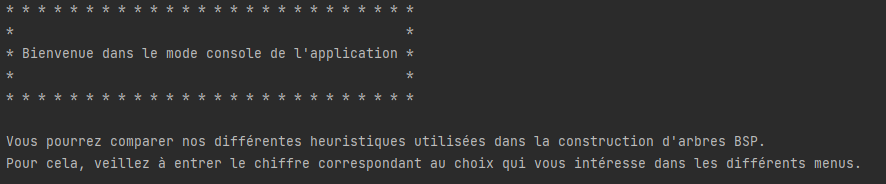
\includegraphics[width=500px]{welcome.png}
  \caption{Message de Bienvenue}\label{fig:PERT}
\end{center}
\end{figure}
\indent On récupère le choix de l'utilisateur avec un Scanner. Si l'utilisateur entre autre chose que les choix proposés, un fichier par défaut sera utilisé: le fichier randomHuge. \\
\begin{figure}[H]
\begin{center}
  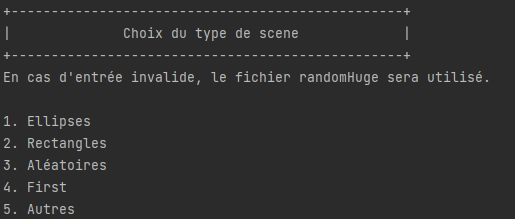
\includegraphics[width=400px]{sceneChoice.png}
  \caption{Choix de la scène}\label{fig:PERT}
\end{center}
\end{figure}
\indent En utilisant un switch sur le choix fait par l'utilisateur, on arrive à l'étape suivante: le choix de la taille de la scene.\\
\indent Comme précedemment, on récupère le choix de l'utilisateur via un scanner et utilisons un switch pour récupérer le path vers le fichier choisi. Pour les fichiers fournit par les enseignants, le path est déjà prêt dans le code. Pour un fichier ajouté manuellement, il y a d'abord la vérification de la conformité et ensuite, si il ne l'est pas, l'application est quittée. \\
\begin{figure}[H]
\begin{center}
  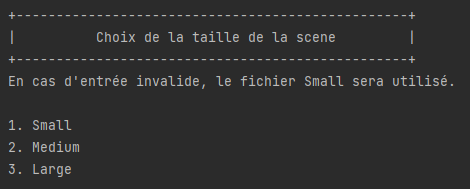
\includegraphics[width=400px]{scizeChoice.png}
  \caption{Choix de la taille}\label{fig:PERT}
\end{center}
\end{figure}
\indent Pour terminer, on imprime quelques informations sur la scene choisie: Son nom, son nombre de segments et la limite de ses axes avant de construire les arbres à partir des différentes heuristiques.\\
\indent Pour chacune d'entre elle, on construit l'arbre et récupérons le temps CPU necessaire pour sa construction grace à la classe Instant de Java, ensuite nous faisons la même chose en effectuant l'algorithme du peintre. \\
\begin{figure}[H]
\begin{center}
  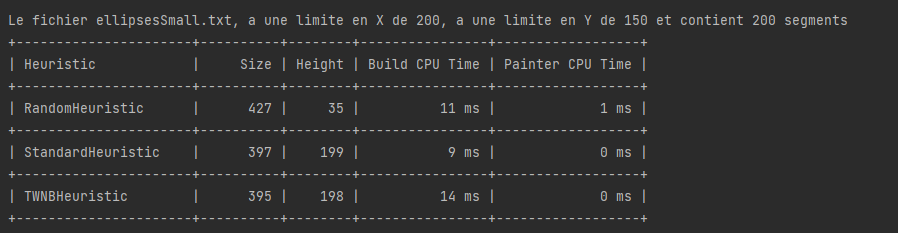
\includegraphics[width=400px]{tree.png}
  \caption{Tableau de résultats}\label{fig:PERT}
\end{center}
\end{figure}
\indent Lorsque toutes les heuristiques ont été faites et que toutes les informations sont regroupées dans un tableau dans la console, on peut soit relancer le même fichier, soit relancer avec un autre fichier, soit quitter l'application. Si l'utilisateur entre autre chose, l'application se fermera.\\
\begin{figure}[H]
\begin{center}
  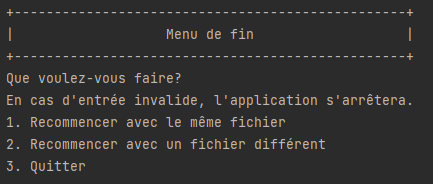
\includegraphics[width=400px]{end.png}
  \caption{Menu final}\label{fig:PERT}
\end{center}
\end{figure}
\indent A tout les endroits où il faut faire un choix, nous avons pensé à faire un choix par défaut en imaginant que l'utilisateur entre autre chose que les dits choix.\\

    {\subsubsection*{5.2.2. L'Algorithme du Peintre en Console (Classe PainterConsole)}}
    \addcontentsline{toc}{subsection}{5.2.2. L'Algorithme du Peintre en Console}
    Dans le mode console, on n'a pas de point de vue. On effectue l'algorithme en incrémentant simplement un compteur à chaque fois que l'on "dessine" un segment. On parcourt chaque noeud de l'arbre.\\
	
    {\subsubsection*{5.2.3. Guide d'utilisation}}
	\addcontentsline{toc}{subsection}{5.2.3. Guide d'utilisation}
	    - Via la console, accéder au dossier ou est le projet\\
	    - Toujours dans la console, compiler le projet à l'aide de la commande gradle build \\
	    - Lancer le mode console via la commande gradle runConsole\\
\indent - Choisir un type de fichier parmi ceux proposés , ou entrer le path vers un fichier externe ajouté via l'invite de commande.\\
\indent - Si un type de fichier à été choisi, choisir sa taille via l'invite de commande.\\
\indent - Recommencer ou non.\\
	
	{\subsection*{5.3. Mode Graphique (Classe TestInteractive)}}
	\addcontentsline{toc}{subsection}{5.3. Mode Graphique}
	
    {\subsubsection*{5.3.1. Implémentation}}
	\addcontentsline{toc}{subsection}{5.3.1. Implémentation}
	
	   {\subsubsection*{5.2.2. L'Algorithme du Peintre graphiquement (Classe PainterInteractive)}}
    \addcontentsline{toc}{subsection}{5.3.2. L'Algorithme du Peintre en Console}
	
    {\subsubsection*{5.3.2. Guide d'utilisation}}
	\addcontentsline{toc}{subsection}{5.3.3. Guide d'utilisation}
	
	
	\newpage 
	{\section*{6. Autres structures de données utilisées}}
	\addcontentsline{toc}{chapter}{6. Autres structures de données}
	Hormis les Arbres BSP, les seules autres structures de données que nous utilisons sont les ArrayList, que l'on utilise pour stocker la liste de segments. Nous les avons choisies car elles sont déjà complètement implémentées dans la bibliothèques java, et sont plus pratiques dans notre cas car au moment de faire la distribution des segments, on ne sait pas combien de segments seront dans l'arbre gauche et l'arbre droit. Les ArrayList n'ayant pas une taille fixe contrairement au tableaux, on pourra sans problème ajouter et supprimer des segments de listes.\\
	Pour les Hashtable, nous ne les avons pas utilisées car nous trouvions les ArrayList assez complètes et simple d'utilisation.\\
			
	{\section*{Conclusion}}
	\addcontentsline{toc}{chapter}{Conclusion}	% to add in the toc	
	

	
	% Appendices
	%\clearpage
	%\appendix		% Changes the numbering of chapters to an alphabetic form and
					% also changes the names of chapters from \chaptername 
					% to the value of \appendixname.
	%\addappheadtotoc	% Makes an entry in the ToC
	%\appendixpage	% Generates a part-like page with the title given by
					% the value of \appendixpagename. 
	
	%\chapter{The first appendix}
	
		


% Back matter
% -----------
%\backmatter			% with class "book" only
	
	% Bibliography
		%\clearpage			% if it does'nt start on a new page
		%\phantomsection	% if any problem with the reference in the toc
	\printbibliography
	%\addcontentsline{toc}{chapter}{Bibliographie}

\end{document}
